\begin{example}[title = Golomb ruler problem]
    e.g. Starting from an empty ruler we have to place $m$ marks. \vspace{7pt}
    \begin{center}
        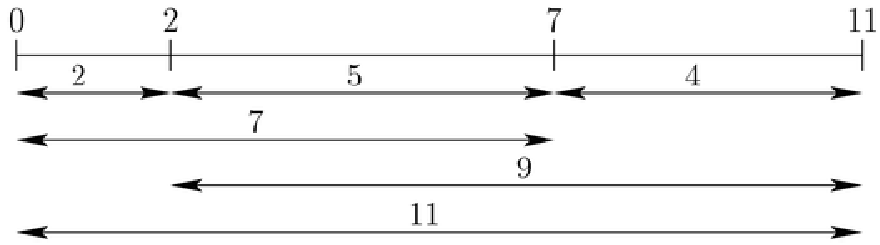
\includegraphics[width = 0.7\textwidth]{img/img6.png}
    \end{center} \vspace{3.5pt}
    At first sight, the problem may appear easy to solve, but instead it's really difficult. Our goal is to place $m$ different marks on a ruler such that 
    the following conditions are satisfied:
    \begin{enumerate}
        \item Distance between each pair of marks is different. 
        \item The length of the ruler obtained is minimum.
    \end{enumerate} \vspace{7pt}

    As shown in the image above, we placed \textit{four marks} over the ruler, achieving a total length equal to $11$, even though this is not the optimal solution. \vspace{3.5pt}
    \begin{center}
        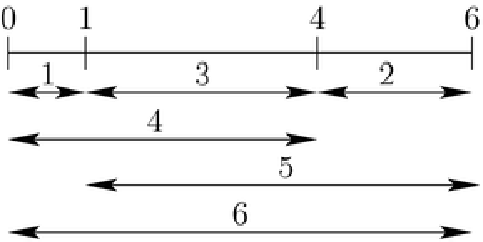
\includegraphics[width = 0.4\textwidth]{img/img7.png}
    \end{center} \vspace{3.5pt}
    With this second approach, we reach a solution up to $6$ always placing \textit{four different marks}. \vspace{7pt}

    \textbf{Decision variables and domains}. \\ 
    It's quite easy to determine the given marks as $m$ different decision variables, but what makes the Golomb ruler problem so difficult is the choice 
    of their domains, in particular:
    \begin{itemize}
        \renewcommand{\labelitemi}{-}
        \item $[X_1, X_2, \dots, X_m]$ are our decision variables.
        \item $\{0, 1, \dots, 2^{m-1}\}$ is the domain of each decision variable. Often the upper limit coincides within $2^{m-1}$, since also in the worst case we are able to place $m$ marks using the powers of $2$, guaranteeing at least one solution.
    \end{itemize} \vspace{7pt}

    \textbf{Constraints}.
    \begin{itemize}
        \renewcommand{\labelitemi}{-}
        \item $\text{for all } i_1 < j_1, i_2 < j_2, i_1 \neq i_2 \text{ or } j_1 \neq j_2 \text{ } |X_{i1} - X_{j1}| \neq |X_{i2} - X_{j2}|$
    \end{itemize}
    Making sure that all pairs of distances have a different difference. \vspace{7pt}

    \textbf{Objective}. \\
    Since we don't know which decision variable will have the highest value, we have to minimize the max value (\textit{the max must be minimum as much as 
    possible}). \vspace{1.5pt} 
    \begin{center}
        $\textit{minimize}(\textit{max}([X_1, X_2, \dots, X_m]))$
    \end{center} \vspace{7pt}

    \textbf{Final mark}. \\
    It's not a good model, since we have absolute values in both sides of the constraint, making hard the propagation. It would be nice to delete these 
    absolute values to get a smoother model. We need to remodel.
\end{example} 
Sometimes we introduce \textbf{additional variables} in our model, even though we said previously more variables we have more large would be the search space.
However, adding variables in order to obtain a bigger search space helps us to express constraints much better than before and, also, spread their propagations.
\begin{example}[title = Better model]
    e.g. Starting from an empty ruler we have to place $m$ marks. \vspace{7pt}

    \textbf{Auxiliary variables}. \\ 
    In the Golomb ruler problem we can introduce a new additional variable $D_{ij}$ that represents the distance between mark $i$ and mark $j$. \vspace{7pt}

    \textbf{Constraints}. \\ 
    The new constraints should be as follows:
    \begin{itemize}
        \renewcommand{\labelitemi}{-}
        \item $\text{for all } i < j, \text{ } D_{ij} = |X_i - X_j|$
        \item $\textit{alldifferent}([D_{12}, D_{13}, \dots, D_{(m-1)m}])$
    \end{itemize}
    Thanks to the additional variable $D_{ij}$ we can directly express a global constraint.
    \begin{itemize}
        \renewcommand{\labelitemi}{-}
        \item $\text{for all } i < j, \text{ } D_{ij} = |X_i - X_j|$
        \item $\textit{alldifferent}([X_1, X_2, \dots, X_m])$
        \item $\textit{alldifferent}([D_{12}, D_{13}, \dots, D_{(m-1)m}])$
    \end{itemize}
    The second constraint introduced is named \textbf{implied constraint}, as the same name suggests, this is a constraint \textbf{logically redundant} but 
    \textbf{computationally significant}. $\textit{alldifferent}([X_1, X_2, \dots, X_m])$ is not a new constraint, since different distances (\textit{the
    third constraint}) already implies that also decision variables $X_1, \dots, X_m$ must be different.
\end{example}